% The "t" in documentclass vertically aligns the frame text to the top
% t-top c-center b-bottom 
\listfiles
\documentclass[croatian,t]{beamer} % must specify a language if using babel
\usetheme{CambridgeUS}
\usecolortheme{beaver}
\usepackage[utf8]{inputenc}
\usepackage{verbatim}
\usepackage{listings}
\usepackage{babel} % đ doesn't work without this package
\usepackage{datetime}
% Changing of bullet foreground color not possible if {itemize item}[ball]
\DefineNamedColor{named}{BrickRed}{cmyk}{0,0.89,0.94,0.28}
\setbeamertemplate{itemize item}[triangle]
\setbeamercolor{title}{fg=BrickRed}
\setbeamercolor{itemize item}{fg=BrickRed}
\setbeamercolor{section number projected}{bg=BrickRed,fg=white}
\setbeamercolor{subsection number projected}{bg=BrickRed}
% Beamer defines "\Tiny" so we have to redefine it to "\tiny"
\let\Tiny=\tiny

\renewcommand{\dateseparator}{.}
\newcommand{\todayiso}{\twodigit\day \dateseparator \twodigit\month \dateseparator \the\year}
\title[NKOSL]{Napredno korištenje operacijskog sustava Linux}
\subtitle{RAID, LVM i kvote}
\author{Goran Cetušić}
\author[Goran Cetušić]{Goran Cetušić\\{\small Nositelj: dr. sc. Stjepan Groš}}
\institute[FER]{Sveučilište u Zagrebu \\
				Fakultet elektrotehnike i računarstva}
\date{\todayiso}

\begin{document}
    %\beamerdefaultoverlayspecification{<+->}
    {
    \setbeamertemplate{headline}[] % still there but empty
    \setbeamertemplate{footline}{}
    \begin{frame}
        \maketitle
    \end{frame}
    }
    
    \begin{frame}
        \tableofcontents
    \end{frame}
    
    \section{Redundant Array of Independent Disks}
	\begin{frame}{RAID}
		\begin{itemize}
			\item RAID omogućava različite kombinacije fizičkog zapisa podataka, najčešće u svrhu očuvanja podataka u slučaju kvara diska
			\item O zapisu se može brinuti
			\begin{itemize}
				\item sklopovlje (hardware RAID) npr. jedan zahtjev kontroleru uzrokovat će identično zapisivanje podataka na dva različita diska
				\item operacijski sustav (software RAID) npr. zapisivanje podataka na particiju znači dupliciranje na dva diska od strane OS-a
			\end{itemize}
			\item Kod odabira vrste RAID-a gledaju se dvije komponente
				\begin{itemize}
					\item Očuvanje podataka
					\item Performanse
				\end{itemize}
			\item Postoji nekoliko teoretskih RAID razina te nekoliko implementacija koje su odbačene npr. RAID 2, 3, 4, 6 i 7
			\item Mi ćemo se baviti samo sa standardnim izvedbama
		\end{itemize}
	\end{frame}    
    
    \begin{frame}{RAID 0}
    	\begin{columns}[c]
    		\begin{column}{6cm}
    			\begin{itemize}
    				\item RAID u tzv. striping modu zapisuje ravnomjerno podatke na dva diska iste veličine
   					\item Ne postoji redundancija podataka - kvar jednog diska znači gubitak svih podataka na njemu
   					\item Zapis podataka je vrlo brz
    			\end{itemize}
    		\end{column}
    		\begin{column}{4cm}
    			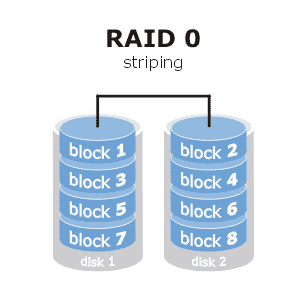
\includegraphics[width=1\textwidth]{../pics/raid0.png}
    		\end{column}
    	\end{columns}
    \end{frame}
    
    \begin{frame}{RAID 1}
    	\begin{columns}[c]
    		\begin{column}{6cm}
    			\begin{itemize}
    				\item RAID u tzv. mirroring modu radi istovjetne kopije na dva diska
   					\item U slučaju kvara jednog diska podaci ostaju zapisani na drugom disku
   					\item Zapis podataka je sporiji jer je potrebno dvaput zapisivati podatke
    			\end{itemize}
    		\end{column}
    		\begin{column}{5cm}
    			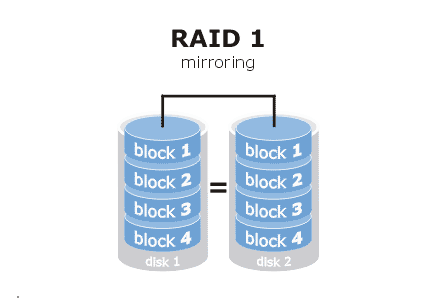
\includegraphics[width=1.2\textwidth]{../pics/raid1.png}
    		\end{column}
    	\end{columns}
    \end{frame}
    
    \begin{frame}{RAID 5}
    	\begin{columns}[c]
    		\begin{column}{6cm}
    			\begin{itemize}
    				\item RAID 5 zapisuje podatke zajedno sa provjerama pariteta
   					\item Potrebna su minimalno 3 diska
   					\item Čitanje podataka je brzo dok je pisanje sporije zbog izračunavanja pariteta
   					\item Ispad bilokojeg diska ne uzrokuje gubitak podataka
    			\end{itemize}
    		\end{column}
    		\begin{column}{5cm}
    			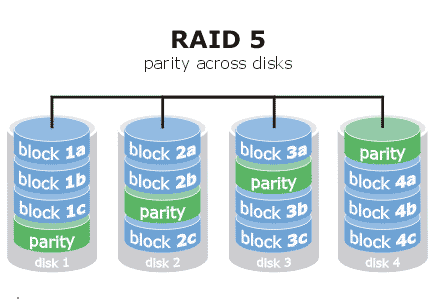
\includegraphics[width=1\textwidth]{../pics/raid5.png}
    		\end{column}
    	\end{columns}
    \end{frame}
    
    \begin{frame}{RAID 10}
    	\begin{columns}[c]
    		\begin{column}{6cm}
    			\begin{itemize}
    				\item Kombinacija RAID 0 i RAID 1
   					\item Dva diska koriste RAID 0 čiji podaci su kopirani na druga dva diska pomoću RAID 1
   					\item Brzina čitanja i pisanja je onakva kakva bi se očekivala istovremenim korištenjem striping i mirroring moda
    			\end{itemize}
    		\end{column}
    		\begin{column}{5cm}
    			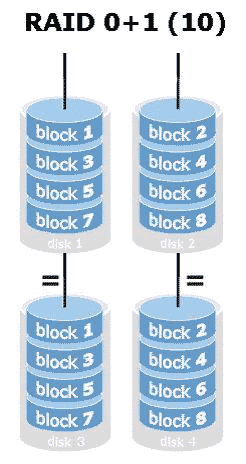
\includegraphics[width=0.6\textwidth]{../pics/raid10.png}
    		\end{column}
    	\end{columns}
    \end{frame}
    
    \begin{frame}[fragile]
	\frametitle{fdisk}
		\begin{itemize}
			\item Particije u RAID-u moraju biti tipa fd (Linux raid auto)
			\begin{lstlisting}[basicstyle={\tiny\ttfamily},language=bash]
Command (m for help): t
Partition number (1-5): 1
Hex code (type L to list codes): L

...
...
16  Hidden FAT16    61   SpeedStor       f2  DOS secondary
17  Hidden HPFS/NTF 63  GNU HURD or Sys fd  Linux raid auto
18  AST SmartSleep  64  Novell Netware  fe  LANstep
1b  Hidden Win95 FA 65  Novell Netware  ff  BBT
Hex code (type L to list codes): fd
Changed system type of partition 1 to fd (Linux raid autodetect)

Command (m for help): p
Disk /dev/hde: 4311 MB, 4311982080 bytes
16 heads, 63 sectors/track, 8355 cylinders
Units = cylinders of 1008 * 512 = 516096 bytes

   Device Boot    Start       End    Blocks   Id  System
/dev/hde1             1      4088   2060320+  fd  Linux raid autodetect
/dev/hde2          4089      5713    819000   83  Linux
/dev/hde4          6608      8355    880992    5  Extended
/dev/hde5          6608      7500    450040+  83  Linux
/dev/hde6          7501      8355    430888+  83  Linux
			\end{lstlisting}
		\end{itemize}
	\end{frame}  
    
    \begin{frame}
    \frametitle{mdadm, mkfs}
    	\begin{itemize}
    		\item Za stvaranje RAID polja se koristi naredba mdadm
    		\begin{scriptsize} \\
mdadm --create --verbose /dev/md0 --level=5  --raid-devices=3 /dev/hde1 /dev/hdf2 /dev/hdg1
			\end{scriptsize}
			\item Inicijalizirana polja mogu se iščitati iz datoteke /proc/mdstat
			\item Nad datotekom /dev/md0 koja predstavlja prvo RAID polje je moguće napraviti datotečni sustav naredbom mkfs
			\begin{itemize}
				\item Da bi radio bio montiran kod podizanja sustava potrebno ga je kao i svaki drugi datotečni sustav dodati u datoteku /etc/fstab
			\end{itemize}
			\item Članovi nekog polja nisu automatski zapamćeni već se njihov popis nalazi u datoteci /etc/mdadm/mdadm.conf na Debian sustavima
			\begin{itemize}
				\item Sintaksa datoteke dobiva se sljedećom naredbom \\
				\begin{scriptsize}
mdadm --detail --scan \\
				\end{scriptsize}
			\end{itemize}
    	\end{itemize}
    \end{frame}
    
    \section{Logical Volume Manager}
    \begin{frame}{LVM}
		\begin{itemize}
			\item LVM pruža fleksibilnije upravljanje skladišnim prostorom od tradicionalnog particioniranja
			\item Često su korisniku potrebne samo tri particije: swap, root i home
			\begin{itemize}
				\item Inače nije moguće raspodijeliti dva diska od 320 GB na particije tako da root particija ima 20 GB a da ostalih 620 GB bude home particija
				\item Moguće je cijeli prvi disk postaviti kao root a drugu kao home particiju
				\item 320 GB je za root particiju je na standardnom sustavu previše
			\end{itemize}
			\item LVM omogućuje spajanje diskova u jednu veliku logičku jednicu od 640 GB te njezino particioniranje po volji
			\item Omogućuje i jednostavno nadodavanje prostora postojećem sustavu
			\begin{itemize}
				\item Dodavanjem diskova
				\item Dodavanjem particija
			\end{itemize}
			\item LVM je moguće definirati tijekom instalacije sustava ili naknadno
		\end{itemize}
	\end{frame}

	\begin{frame}{Scenarij}
		\begin{itemize}
			\item Home particija je postala puna i potrebno je dodati više prostora sustavu. 
			\begin{itemize}
				\item Na raspolaganju imamo samo jedan dodatni disk koji je manji od trenutnog.
				\item Kopiranje podataka sa trenutnog diska na manji nije opcija jer time dobivamo još manje prostora za podatke.
				\item Na raspolaganju imamo samo jedan dodatni disk koji je manje od trenutnog.  /dev/sda je disk koji sadrži home particiju /dev/sda5, dok je drugi manji disk /dev/sdb sa particijom /dev/sdb1.
			\end{itemize}
			\item Standardno rješenje u ovom slučaju je LVM			
		\end{itemize}
	\end{frame}		
	\begin{frame}{LVM pojmovi}
		\begin{itemize}
			\item Physical Volume (PV)
			\begin{itemize}
				\item Drugi naziv za disk ili particiju koji će biti dio veće jedinice
			\end{itemize}
			\item Volume Group (VG)
			\begin{itemize}
				\item Nekoliko PV-a će biti grupirano u VG
				\item U kontekstu LVM-a ovo predstavlja virtualni disk 
			\end{itemize}
			\item Logical Volume (LV)
			\begin{itemize}
				\item VG se mogu podijeliti na manje logičke jedinice - LV
				\item U kontekstu LVM-a ovo predstavlja particije
			\end{itemize}
			\item Physical Extent (PE)
			\begin{itemize}
				\item LVM dijeli svaki disk na manje jedinice - PE
				\item Možemo ih zamisliti kao sektore na fizičkim diskovima
				\item Standardna veličina je 4 MB
			\end{itemize}
			\item Logical Extent (LE)
			\begin{itemize}
				\item Kao PE ali za LV-ove
				\item Njihova veličina je jednaka veličini PE
			\end{itemize}
		\end{itemize}	
	\end{frame}	

	\begin{frame}
    	\begin{columns}
    		\begin{column}{4cm}
    			\begin{figure}
					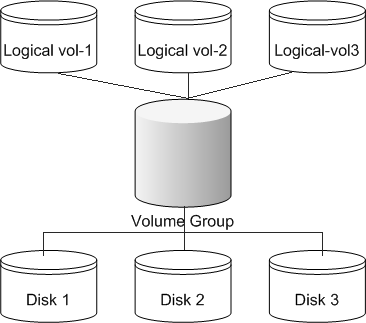
\includegraphics[width=1.2\textwidth]{../pics/lvm.png}
				\end{figure}
			\end{column}
			\begin{column}{4cm}
				\begin{figure}
					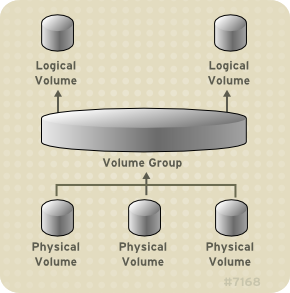
\includegraphics[width=1.2\textwidth]{../pics/basic-lvm-volume.png}
				\end{figure}
			\end{column}
		\end{columns}
    \end{frame}

	\begin{frame}[fragile]
	\frametitle{fdisk}
		\begin{itemize}
			\item Prvo je potrebno odmontirati korištene particije
			\item Nakon toga se tip particije mora promijeniti u 8e (Linux LVM)
			\begin{itemize}
				\item Najjednostavniji način je korištenjem fdisk naredbe			
			\end{itemize}
			\begin{itemize}
				\item Ovdje je vidljivo čemu služe tipovi particija
				\item OS koristi LVM za spajanje particija u jednu cjelinu
			\end{itemize}
		\begin{lstlisting}[basicstyle={\tiny\ttfamily},language=bash]
Command (m for help): p
 
Disk /dev/hde: 4311 MB, 4311982080 bytes
16 heads, 63 sectors/track, 8355 cylinders
Units = cylinders of 1008 * 512 = 516096 bytes
 
   Device Boot    Start       End    Blocks   Id  System
/dev/sda1             1      4088   2060320+  fd  Linux raid autodetect
/dev/sda2          4089      5713    819000   83  Linux
/dev/sda3          5714      6607    450576   83  Linux
/dev/sda4          6608      8355    880992    5  Extended
/dev/sda5          6608      7500    450040+  8e  Linux LVM
		\end{lstlisting}		
		\end{itemize}
	\end{frame}	
	
	\begin{frame}[fragile]
	\frametitle{pvcreate, vgcreate, vgscan}
		\begin{itemize}
			\item Sve PV-ove moramo tako definirati
			\item Oprez! Ovo briše podatke na particijama!
			\begin{lstlisting}[basicstyle={\tiny\ttfamily},language=bash]
sh-2.05b# pvcreate /dev/sda5 /dev/sdb1
pvcreate -- physical volume "/dev/sda5" successfully created
pvcreate -- physical volume "/dev/sdb1" successfully created
sh-2.05b#
			\end{lstlisting}
			\item Od PV-ova se mora složiti VG
			\begin{lstlisting}[basicstyle={\tiny\ttfamily},language=bash]
sh-2.05b# vgcreate lvm-disk /dev/sda5 /dev/sdb1
Volume group "lvm-disk" successfully created
sh-2.05b#
			\end{lstlisting}
			\item Bilo bi dobro provjeriti je li grupa uistinu stvorena
			\begin{lstlisting}[basicstyle={\tiny\ttfamily},language=bash]
sh-2.05b# vgscan
vgscan -- reading all physical volumes (this may take a while...)
Found volume group "lvm-disk" using metadata type lvm2
sh-2.05b#
			\end{lstlisting}
		\end{itemize}
	\end{frame}
	
	\begin{frame}[fragile]
	\frametitle{pvdisplay, vgdisplay}
		\begin{itemize}
		\item Dodatne naredbe: pvdisplay, vgremove, vgrename, lvextend, lvreduce, lvscan, lvremove, lvrename...
		\item vgdisplay ispisuje informacije o specifičnoj grupi
			\begin{lstlisting}[basicstyle={\tiny\ttfamily},language=bash]
sh-2.05b# vgdisplay lvm-disk
--- Volume group ---
VG Name               lvm-disk
VG Access             read/write
VG Status             available/resizable
VG #                  0
MAX LV                256
Cur LV                0
Open LV               0
MAX LV Size           255.99 GB
Max PV                256
Cur PV                2
Act PV                2
VG Size               848 MB
PE Size               4 MB
Total PE              212
Alloc PE / Size       0 / 0
Free  PE / Size       212 / 848 MB
VG UUID               W7bgLB-lAFW-wtKi-wZET-jDJF-8VYD-snUaSZ
			\end{lstlisting}
		\end{itemize}
	\end{frame}

	\begin{frame}[fragile]
	\frametitle{lvcreate}
		\begin{itemize}
			\item Posljednja LVM naredba prije stvaranja datotečnog sustava je lvcreate
			\item Stvaranje LV-a navođenjem broja PE
			\begin{lstlisting}[basicstyle={\tiny\ttfamily},language=bash]
sh-2.05b# lvcreate -l 212 lvm-disk -n lvm0
Logical volume "lvm0" created
sh-2.05b#
			\end{lstlisting}
			\item Stvaranje LV-a od svog slobodnog prostora grupe
			\begin{lstlisting}[basicstyle={\tiny\ttfamily},language=bash]
sh-2.05b# lvcreate -l 100%FREE -n lvm0 lvm-disk
			\end{lstlisting}
			\item Stvaranje LV-a od pola sveukupnog prostora grupe
			\begin{lstlisting}[basicstyle={\tiny\ttfamily},language=bash]
sh-2.05b# lvcreate -l 50%VG -n lvm0 lvm-disk
			\end{lstlisting}
			\item I na kraju stvaranje datotečnog sustava na logičkom jedinicom
			\begin{lstlisting}[basicstyle={\tiny\ttfamily},language=bash]
sh-2.05b# mkfs -t ext3 /dev/lvm-disk/lvm0
			\end{lstlisting}
			\begin{itemize}
				\item Primijetite imena direktorija grupe i pripadajuće datoteke za LV unutar /dev direktorija
			\end{itemize}
		\end{itemize}	
	\end{frame}
	
    \section{Kvote}
	\begin{frame}[fragile]
	\frametitle{Vrste kvota}
		\begin{itemize}
			\item Kvote ograničavaju zauzeće diska po korisniku ili grupi
			\begin{itemize}
				\item usrquota - kvote se definiraju po korisniku npr. svaki korisnik ima kvotu od 30 GB
				\item grpquota - kvote se definiraju po grupi npr. zajednička kvota svih korisnika u nekoj grupi je 500 GB
			\end{itemize}
			\item Ovo su "obične" kvote, kernel podržava i tzv. \textit{journaled} kvote
			\begin{itemize}
				\item usrjquota, grpjquota
				\item Velika prednost je što se ne proračunavaju kvote kod podizanja sustava što čini proces bržim
			\end{itemize}
			\item Ako dobijete sljedeću poruku tijekom stvaranja kvota kernel podržava \textit{journaled} kvote
			\begin{lstlisting}[basicstyle={\tiny\ttfamily},language=bash]
quotacheck: Your kernel probably supports journaled quota but you are not using it.
Consider switching to journaled quota to avoid running quotacheck after an unclean
shutdown.
			\end{lstlisting}
		\end{itemize}
	\end{frame}

	\begin{frame}[fragile]
	\frametitle{Naredbe}
		\begin{itemize}
			\item \textit{quotaon} - uključivanje kvota
			\item \textit{quotaoff} - isključivanje kvota
			\item \textit{edquota} - mijenjanje kvota
			\item \textit{repquota} - ispisivanje kvota po korisniku
			\item \textit{quotacheck} - osvježavanje baze
			\begin{itemize}
				\item zapisuje stanje kvota za ostale programe
			\end{itemize}
			\item Provjera podrške za kvote u kernelu:
			\begin{lstlisting}[basicstyle={\tiny\ttfamily},language=bash]
# grep -i config_quota /boot/config-`uname -r`
CONFIG_QUOTA=y
CONFIG_QUOTACTL=y
			\end{lstlisting}
		\end{itemize}
	\end{frame}
	
	\begin{frame}[fragile]
	\frametitle{Instalacija}
		\begin{itemize}
			\item Instalacija \textit{userspace} alata
			\begin{lstlisting}[basicstyle={\tiny\ttfamily},language=bash]
apt-get install quota
			\end{lstlisting}
			\item Omogućavanje kvota za particiju u /etc/fstab
		\end{itemize}
		\begin{lstlisting}[basicstyle={\tiny\ttfamily},language=bash]
# ... <options> 	<dump> 		<pass>
... errors=remount-ro,usrjquota=aquota.user,grpjquota=aquota.group,jqfmt=vfsv0 0 1
		\end{lstlisting}
		\begin{itemize}
			\item Stvaranje datoteka za kvote i ponovno montiranje particija
			\begin{itemize}
				\item aquota.user i aquota.group moraju biti točno u onom direktoriju u koji je montirana particija npr. /home u ovom slučaju a ne u poddirektoriju
			\end{itemize}
			\begin{lstlisting}[basicstyle={\tiny\ttfamily},language=bash]
touch /home/aquota.user /home/aquota.group
chmod 600 /home/aquota.*
mount -o remount /home
			\end{lstlisting}
			\item Izračunavanje kvota i uključivanje
			\begin{itemize}
				\item Moguće je uključiti sve particije ili pojedinačno
			\end{itemize}
			\begin{lstlisting}[basicstyle={\tiny\ttfamily},language=bash]
quotacheck -avugm
quotaon -avug
			\end{lstlisting}
		\end{itemize}
	\end{frame}
	
	\begin{frame}[fragile]
	\frametitle{Limit}
		\begin{itemize}
			\item Kvote za pojedinačnog korisnika ili grupu mogu ima \textit{hard} i \textit{soft} limit
			\begin{itemize}
				\item soft limit - nakon dostignutog limita korisnik ima \textit{grace} vrijeme tijekom kojeg može i dalje puniti disk pod uvjetom da ne dostigne hard limit
				\item hard limit - korisnik ne može ni pod kojim uvjetima prijeći ovaj limit
			\begin{lstlisting}[basicstyle={\tiny\ttfamily},language=bash]
# repquota -a

*** Report for user quotas on device /dev/md0
Block grace time: 7days; Inode grace time: 7days
                        Block limits                File limits
User            used    soft    hard  grace    used  soft  hard  grace
----------------------------------------------------------------------
root      --      52       0       0             10     0     0       
veljko    -- 25585028 40000000 40000000           1123     0     0       
cetko     -- 5162460 40000000 40000000             49     0     0       
marin     -- 6498572 10000000 20000000            183     0     0       
deni      -- 5903852 10000000 20000000            528     0     0       
lovro     -- 3649796 10000000 20000000             19     0     0       
matej     +- 11334792 10000000 20000000  2days     646     0     0       
			\end{lstlisting}	
			\end{itemize}
		\end{itemize}
	\end{frame}
	
	\begin{frame}[fragile]
	\frametitle{Mijenjanje i postavljanje}
		\begin{itemize}
			\item Naredba \textit{edquota} otvara preferirani editor korisnika za mijenjanje kvota
		\end{itemize}
		\begin{lstlisting}[basicstyle={\tiny\ttfamily},language=bash]
# edquota cetko

Disk quotas for user cetko (uid 1001):
  Filesystem                   blocks       soft       hard     inodes     soft     hard
  /dev/md0                    5162460   40000000   40000000         49        0        0     
		\end{lstlisting}
		\begin{itemize}
			\item U datoteci /etc/adduser.conf je moguće definirati postojećeg korisnika prema kojem će novom korisniku biti postavljene kvote
			\begin{lstlisting}[basicstyle={\tiny\ttfamily},language=bash]
.
.
.
# If QUOTAUSER is set, a default quota will be set from that user with
# `edquota -p QUOTAUSER newuser'
QUOTAUSER="pesha"
			\end{lstlisting}
		\end{itemize}
	\end{frame}	
	
	\section{}
	\begin{frame}{Literatura}
		\begin{tiny}
			\url{http://www.raids.co.uk/} \\
			\url{http://www.prepressure.com/library/technology/raid} \\
			\url{http://docs.hp.com/en/B2355-90672/ch03s06.html} \\
			\url{http://tldp.org/HOWTO/LVM-HOWTO/} \\
			\url{http://unixfoo.blogspot.com/2008/12/linux-logical-volume-manager-basics.html} \\
			\url{http://www.howtoforge.com/linux_lvm} \\
			\url{http://www.yolinux.com/TUTORIALS/LinuxTutorialQuotas.html} \\
			\url{http://linuxhelp.blogspot.com/2005/10/disk-quotas-in-linux-explained.html} \\
		\end{tiny}
	\end{frame}
\end{document}
